%\documentclass{vldb}

\documentclass[conference]{IEEEtran}

\usepackage{url}
\usepackage{graphicx}
\usepackage{subfigure}
\usepackage{balance}  % for  \balance command ON LAST PAGE  (only there!)
\usepackage{algpseudocode,algorithm}
\usepackage{epstopdf}

\newcommand{\eat}[1]{}


\begin{document}

% ****************** TITLE ****************************************

\title{FrugalDB: A Cost-Efficient Multi-Tenant Database System }

\author{
Yifeng Luo $^{\S 1}$, Junshi Guo $^{\S 2}$, Jiaye Zhu $^{\S 3}$, Zhenjie Zhang $^{\dag 4}$, Shuigeng Zhou $^{\S 5}$
\vspace{1.6mm}\\
\fontsize{10}{10}\selectfont\itshape
$^{\dag}$ School of Computer Science, Fudan University, China P.R.\\
\fontsize{9}{9}\selectfont\ttfamily\upshape
$^{1,2,3,5}$\{luoyf,jsguo14,zhujy14,sgzhou\}fudan.edu.cn
\vspace{1.2mm}\\
\fontsize{10}{10}\selectfont\rmfamily\itshape
$^{\dag}$Advanced Digital Sciences Center, Illinois at Singapore Pte. Ltd., Singapore \\
\fontsize{9}{9}\selectfont\ttfamily\upshape
$^{4}$zhenjie@adsc.com.sg
}


\maketitle

\begin{abstract}
Quality of Service~(QoS) is at the core of the vision in Database as a Service~(DBaaS), which provides guarantees to the database users on the usability of the database service, even when the underlying database infrastructure is shared by multiple users. Traditional approaches in DBaaS reserve computation resources, e.g. CPU and memory, based on the Service Level Objective~(SLO) given by the database users, so that the database engine always possesses sufficient resource to accomplish the expected workload under any circumstance. Such resource reservation schemes inevitably result in poor resource utilization, as the actual workload of the tenants are usually way below their maximal workload expectation described in their SLO.

To enhance resource utilization and reduce operational cost, we propose a novel architecture in our prototype multi-tenant database system, \emph{FrugalDB}, which generally consolidates more tenants with performance SLOs on one single database server. FrugalDB accommodates two independent database engines, an in-memory engine for high workloads with tight SLOs, and a disk-based engine for less active workload with loose SLOs. The dual processing logic enables huge computation resource saving, by assigning the workloads from the tenants to the appropriate engine for query processing. Different from traditional multi-tenant database system, the design of FrugalDB put emphasis on the migration cost minimization, which is incurred when moving workloads across the engines. Based on a workload estimation, FrugalDB responds quickly to the workload updates with minimal overhead on database migration. We validate and evaluate FrugalDB with extensive experiments, which proves its prohibitively higher tenant consolidation rate with performance SLO guarantees, fewer performance SLO violations and acceptable response latency.
\end{abstract}


\section{Introduction}\label{sec:Introduction}

%As big data techniques and infrastructures are being applied to facilitate and accelerate the processing of big data with formidable size, people are putting forward eager requests on (quasi-)real-time processing of big datasets yet with exploding volumes, while meeting the (quasi-)real-time processing requests of big datasets is held back by the disk-based storage subsystem, because of the expanding tremendous performance gap lying between magnetic disks and processing units.

Memory caching \textcolor{red}{plays} a crucial role in bridging the performance gap between \textcolor{red}{storage subsystems and computing frameworks, which gradually becomes the determinant of whether processing units of big data platforms could work at wire speed to satisfy people's growing computing requirements.}
As more and more time-critical applications commence employing memory to cache datasets, big data clusters \textcolor{red}{are usually} shared by multiple computing \textcolor{red}{frameworks}, applications or end users, and  there exists intense competition for memory cache resources, especially on small clusters which are supposed to 
\textcolor{red}{process comparably big datasets as large clusters do, yet with tightly limited resources.}
Consequently implementing effective and adaptive management on memory cache resources becomes increasingly important for the efficient running of big data clusters, especially for small/medium enterprises \textcolor{red}{who} could only afford to build non-big clusters. Applying existing on-demand caching strategies on small shared clusters inevitably results in frequent cache thrashings when the conflicts of simultaneous cache resource demands are not mediated, \textcolor{red}{leading to deterioration in overall cluster efficiency.}
The principal reason is that aggressively caching massive number of data blocks of big datasets on demand causes \textcolor{red}{constant block replacement in cache, and thus conversely exacerbates resource competition.}

%\begin{figure}[!htb]
%\centering
%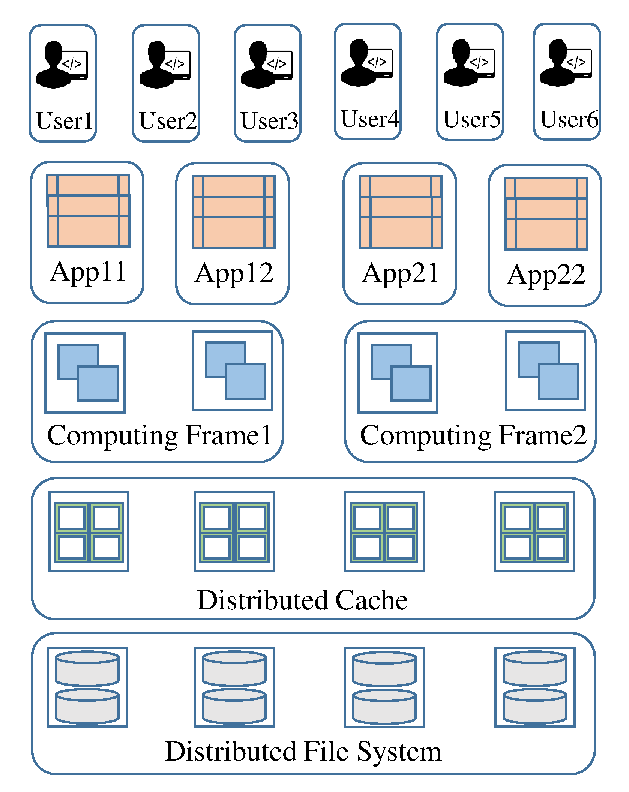
\includegraphics[width=0.4\textwidth]{figures-final/Hierarchy.eps}
%\caption{Big data application hierarchies.}
%\label{fig:hierarchy}
%\end{figure}

%Intense competition for computational resources would do no harm to the clusters' running efficiency, while intense competitions for memory cache resources may incur frequent cache thrashings if cache resource demands are not coordinated, which would engender tremendous harm to the clusters' running efficiency.

%Applying existing on-demand caching strategies, which cache in data blocks once they are accessed, on small shared clusters could not prevent cache thrashings when the conflicts of simultaneous cache resource demands are not mediated. The principal reason is that aggressively caching massive number of data blocks of big datasets on demand causes constantly block replacement in cache, and thus exacerbates the competition of memory cache resources when these resources are in strong need.

\textcolor{red}{Web or traditional OLTP database applications usually produces vast difference in range or block "hotness" regarding access recency and frequency. Though in big data applications, input files are usually scanned as a whole for data processing and all blocks reveal almost equal "hotness".}
%Unlike Web or traditional OLTP database applications, where various ranges or blocks of the same dataset may possess \textcolor{red}{vast} different "hotness", regarding access recency and frequency of blocks, big data applications usually scan their input files for data processing as a whole, and all blocks of a file thus possess almost the same level of "hotness". 
\textcolor{red}{On the other hand}, traditional \textcolor{red}{system-level} or database-level data caching is executed on small data units (i.e. 8KB-sized pages), while big data caching is executed on \textcolor{red}{much larger} units(i.e. 256MB-sized blocks). So the cost of caching in/out a data unit \textcolor{red}{in big data scenarios} far exceeds that \textcolor{red}{of} traditional data caching. Accordingly, traditional caching may have millions of \textcolor{red}{cache slots}, and this makes hotter data less likely cached out by colder data; while big data caching may only have thousands of slots, which \textcolor{red}{shows almost no preference for particular slots.}
%makes hotter data vulnerable to being cached out by colder data.

Targeting the caching problem existing on non-big clusters, we propose an adaptive cache mechanism, which is named as EARNCache~(from s\textbf{E}lf-\textbf{A}daptive inc\textbf{R}eme\textbf{N}tal \textbf{Cache}), to coordinate concurrent cache resource demands to prevent exacerbated cache efficiency \textcolor{red}{\sout{in this paper}}, when intense competitions for memory cache resources occur. As big data applications usually access their input data in Write-Once-Read-Many~(WORM) fashion, we only consider read caching in this paper. Major contributions of this paper include: ~1) proposing an incremental caching mechanism which could self-adaptively adjusts cache allocation strategies according to the competition condition of cache resources; ~2) formulating and solving the cache resource allocation and replacement problem as an optimization problem; ~3) implementing a prototype of the proposed method, and performing extensive experiments to evaluate the effectiveness of \textcolor{red}{the proposed mechanism.}
%incremental big data caching mechanism.

%With EarnCache, applications or end users incrementally earn cache resources from other applications or end users by accessing their datasets, where a dataset is cached gradually as the upper-level application or end users earns more and more resources, but not cached as a whole on demand.

In the rest of this paper, we first illustrate the system design and implementation details of EARNCache in Sec.~\ref{sec:SDI}. We provide empirical results in Sec.~\ref{sec:Experiments}, and present the related work in Sec.~\ref{sec:RelatedWork}. We finally conclude the paper in Sec.~\ref{sec:Conclusion}.


\section{Related Work}\label{sec:RelatedWork}

There has been extensive work on memory storage and caching, as more and more time-critical applications~\cite{redis,memcached} require to store or cache data in memory to gain improved data access performance, such as J. Ousterhout, et al proposed RAMCloud~\cite{ramcloud} to keep data entirely stored in memory for large-scale Web applications, and Spark~\cite{spark,rdd} enables in-memory MapReduce~\cite{mapreduce}-style parallel computing by leveraging memory to store and cache distributed (intermediate) datasets.

%While caching on distributed parallel systems is tremendously different from traditional centralized page-based file system or database caching, and directly applying centralized caching usually does not help much to improve and sometimes even hurts cache efficiency and performance.

Some previous work focuses on implementing an additional layer on existing distributed file system, which enables applications to cache distributed datasets from the underlying distributed file system. J. Zhang, et al.~\cite{dist-cache-hdfs} and Y. Luo, et al.~\cite{rcss} respectively proposed the HDCache and RCSS distributed cache system based on HDFS~\cite{hdfs1,hdfs2}, which manages cached data just as HDFS manages disk data. H. Li, et al.~\cite{tachyon} further implemented a distributed memory file system for data caching by checkpointing data to the underlying file system. EARNCache imbeds the incremental caching into Tachyon~\cite{tachyon} to coordinate resource competitions and avoid cache thrashings, and improves cache efficiency and resource fairness to a certain degree.

Some work focuses on optimizing data caching for specific frameworks or goals. S. Zhang, et al.~\cite{mapreduce-cache} proposed to cache MapReduce intermediate data to speed up MapReduce applications. G. Ananthanarayanan, et al.\cite{pacman} found the important All-or-Nothing property, which implies all or none input data blocks of tasks within the same wave should be cached, and then proposed PACMan to coordinate memory caching for parallel jobs. Y. Li, ~et al.\cite{rate-aware}, S. Tang, et al.~\cite{ltrf} and A. Ghodsi, et al.~\cite{drf} respectively proposed dynamic resource partition strategies to improve fairness, and maximize the overall performance in the meanwhile. Q. Pu, et al.~\cite{fairride} extended the MAX-MIN fairness~\cite{maxmin,maxmin2} with probabilistic blocking, and proposed FairRide to avoid cheating and improve fairness for shared cache resources.



\renewcommand{\algorithmicrequire}{\textbf{Input:}}
\renewcommand{\algorithmicensure}{\textbf{Output:}}

\section{System Framework}\label{sec:SDI}
We mainly illustrate how \textcolor{red}{EARNCache} works in this section. Firstly we present the overview about the cache-earning mechanism of \textcolor{red}{EARNCache}, and then illustrate its architecture design, and finally explains the incremental cache-earning policy and its implementation.

\subsection{Overview}\label{sec:overview}

On shared non-big clusters with relatively limited cache capacity, cache resource conflicts \textcolor{red}{\sout{on non-big clusters}} would be \textcolor{yellow}{norm rather than exception}. When only quite few users are using a non-big cluster and the competition for cache resources is mild, applying on-demand caching could expedite hotter blocks taking over cache resources from colder blocks, and hotter data is less likely to be cached out by colder data. When more concurrent users are using the cluster and the competition for cache resources gets wild, on-demand caching leaves concurrently cache resource demands unmediated, which makes hotter data more vulnerable to being cached out. Files which are frequently accessed recently sometimes could be totally cached out by files which would rarely be accessed for the second time in the near future, then these hot cached-out files need caching in soon as their next access should occur in the incoming future. We consequently need to revisit existing on-demand caching mechanisms and strategies, and propose more effective measures to improve the efficiency of data caching on non-big clusters.

We believe that a good caching strategy for non-big clusters should be self-adaptive to resource competition conditions to depress competitions and avoid thrashings when resources are in desperate deficit. Obviously caching big data files on demand as a whole could not provide such self-adaptivity. Intuitively we should not cache files entirely \textcolor{red}{\sout{when caching them entirely causes tension. }}
Not compulsorily caching files entirely provides the elasticity of tuning the amount of cache resources allocated for different files, according to the files' access recency and frequency.

Ideally, more \textcolor{red}{recently frequently accessed files} should be assigned with more cache resources, \textcolor{red}{and less recently frequently accessed files}
%and less frequently accessed files recently 
should be assigned with less cache resources. However, \textcolor{red}{it's not possible to know in advance what files would be frequently accessed in the upcoming future and we could only make predictions based on historical file access patterns, especially the most recent information.}
%it's impossible to know for sure what files would be frequently accessed files recently, and we could only make predictions based on available historical file access information, especially recent accesses. 
Based on files' historical access information, \textcolor{red}{EARNCache} implements an incremental caching strategy, where a user should earn resources to cache files from other concurrent users via accessing these files. Cache resources are incrementally allocated to files becoming frequently accessed, which gradually takes over cache resources from files getting less frequently accessed, until all blocks of the file have been cached in. The more a \textcolor{red}{file} is accessed, the more cache resources it takes over. The incremental caching strategy ensures that cached hot files being frequently accessed recently will not be flushed out by other massive less hot files, which may only be accessed occasionally or randomly.

\subsection{Architecture}\label{sec:Arch}
Cached files originally are stored in the under distributed file system (i.e. Hadoop File System), and \textcolor{red}{EARNCache} \textcolor{red}{\sout{globally}} coordinately cache them across the whole cluster. \textcolor{red}{EARNCache}'s architecture consists of a central \emph{master} and a set of \emph{workers} residing on storage nodes of the cluster(see Fig.~\ref{fig:Arch}). 
The master's main role is: ~1) to determine how many cache resources should be allocated to a file, based on the resource competitions; ~2) to inform workers of cache resource allocation plans via heartbeats; ~3) to \textcolor{red}{keep} track of cache metadata about which storage node a cached block resides on; ~4) to answer clients' queries on cache metadata. \textcolor{red}{And} the worker's main role is: ~1) to receive resource allocation plans from the master; ~2) to calculate how many resources a file should contribute to compose the allocated resources; ~3) to cache in/out blocks according to the calculated resource composition plans; ~4) to inform the master of cached blocks via heartbeats; ~5) serve clients with cached blocks.

The procedures of a client accessing a block are: ~1) the client queries the master where the block is located; ~2) the master tells the client which worker it should contact to access the block; ~3) the client contacts the worker to access the block; ~4) the worker serves the client with the block data from cache. One thing worth noting here is that: the client will not contact any worker to access a block if the block has been cache out, as the master only keeps track of cached blocks, and could not provide the client with information about \textcolor{red}{cached-out blocks}, then the client has to turn to the under file system for this block.


\begin{figure}[!htbp]
\centering
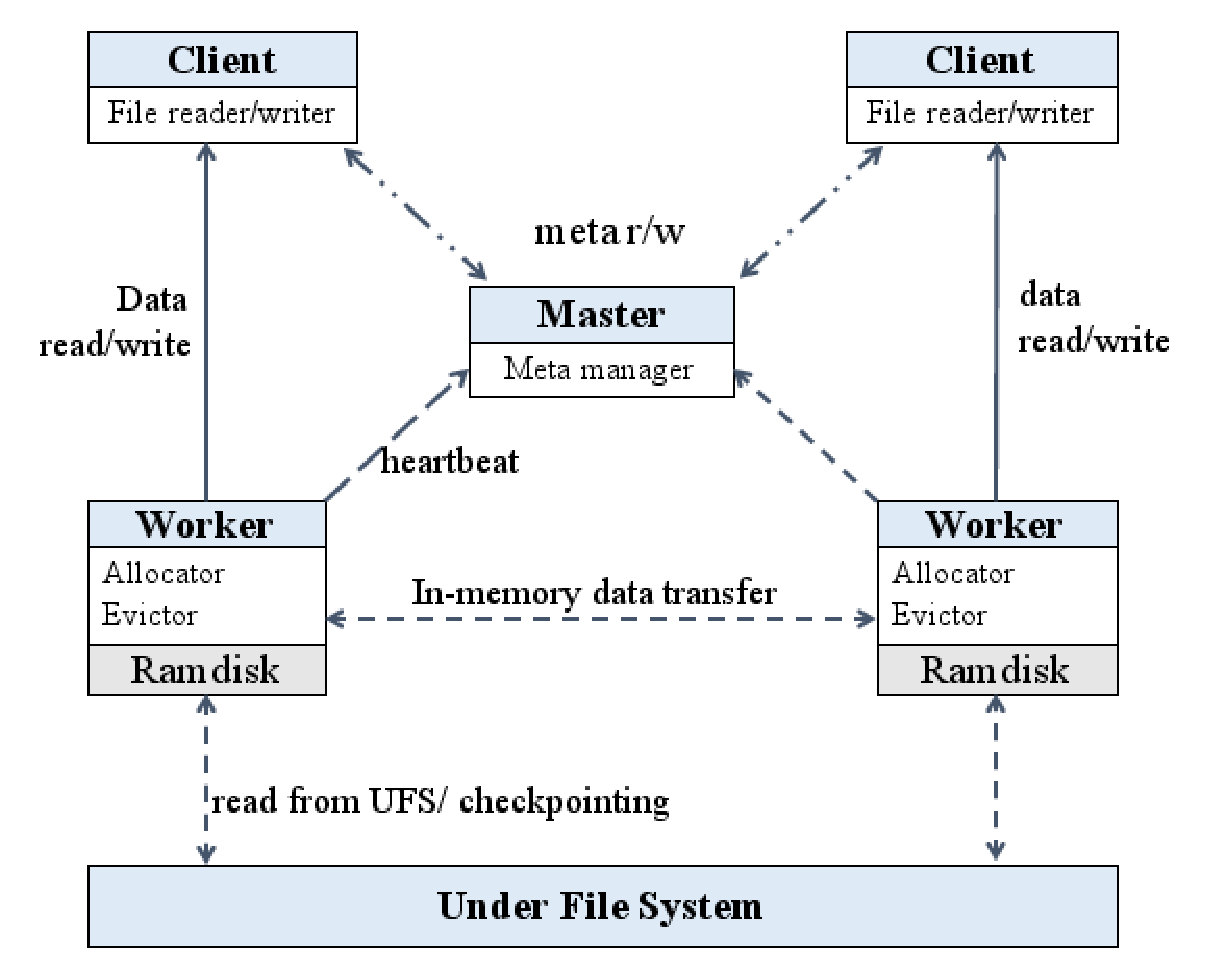
\includegraphics[scale=0.4]{figures/architecture.eps}
\caption{EARNCache's Architecture.}
\label{fig:Arch}
\end{figure}

%Competition for computational resources rarely influences the completion of running tasks, namely each of the scheduled concurrent tasks may run as fast as it runs alone. does not have obviously decrease computation efficiency, as ; while competition for cache resources may seriously decrease cache efficiency, because of data caching in/out cost.
%Big data applications usually access files in a scan fashion and datasets are usually prohibitively huge in size.
%Work about on-demand caching mainly focuses on cache replacement policies, and most replacement policies are variants of LRU, LFU or LRU-LFU-combined.

\subsection{Incremental Caching}\label{sec:framework master}

As we prefer to letting frequently accessed files recently incrementally take over resources from less frequently accessed files recently, "recently" should be defined quantitatively before we could design the incremental caching strategy, and other related elements should also be defined. Tab.~\ref{tab:notation} presents all definitions of notations involved in our incremental caching strategy.
\begin{table}[!htb]
	\caption{Notation definitions}
	\label{tab:notation}
	\centering
	\begin{tabular}{|p{0.15\linewidth}|p{0.75\linewidth}|}
		\hline
		Notation & Definition\\
		\hline
		$W$ & predefined window size of the most recently accessed data for observing files falling within\\
		\hline
		$a,b$ & scan time per unit data from memory(a) and hdd(b) \\
		\hline
		$N$ & total number of files falling in the observation window\\
		\hline
		$d_i$ & data size of the $i$th file\\
		\hline
		$D$ & total data size of $N$ files\\
		\hline
		$M$ & cache capacity of the whole cluster\\
		\hline
		$f_i$ & access frequency of the $i$th file\\
		\hline
		$F$ & total access frequency of $N$ files\\
		\hline
		$x_i$ & percentage of data cached for the $i$th file\\
		\hline
		$h_i(x_i)$ & the $i$th file's profit gain with $x_i$ data cached\\
		\hline
	\end{tabular}
\end{table}

We define a function $h_i(x_i)$ to denote the profit gain of the $i$th file to instruct how cached files should contribute resources. Then we attempt to instantiate $h_i(x_i)$ and to maximize total profit gain of all files falling in the observation window, just as Equ.\ref{optimization target} shows.
\begin{equation}\label{optimization target}
\sum_{i=1}^{N} f_i \cdot h_i(x_i) \
\end{equation}

According to definitions in Tab.\ref{tab:notation}, we can assume that the time it takes to scan the $i$th file is:
\begin{equation}\label{time}
time(x_i)=[a\cdot x_i+b\cdot (1-x_i)]\cdot d_i
\end{equation}

As mentioned above, we use $h_i$ to indicate the $i$th file's profit gain with $x_i$ data cached. If we take saved scan time as a file's profit gain, then we can define $h_i$'s deviation at $x_i$ as its gain change over $\delta x_i$, which could be further defined as the percentage of increased saving of the file's scan time with increased cache share at $x_i$ over the total saved scan time at $x_i$, compared to zero cache share, just formulized as:
\begin{equation}\label{dhi}
\frac{\delta h_i}{\delta x_i}=\frac{time(x_i) - time(x_i+\delta x_i)}{time(0) - time(x_i)}=\frac{\delta x_i}{x_i}
\end{equation}

Thus we can derive that $h_i(x_i)=\ln x_i$, and now our optimization goal becomes
\begin{equation}
\sum_{i=1}^{N} f_i \cdot \ln x_i
\end{equation}
subjected to
\begin{equation}
\sum_{i=1}^{N} x_i\cdot d_i \leq M
\end{equation}

Note at any given time,  $x_i$ is the only variant contained in the optimization goal, and $f_i \cdot \ln x_i$ is a convex function. After applying Lagrange multiplier method, our maximizing goal turns to:
\begin{equation}
L=\sum_{i=1}^{N} f_i\cdot \ln x_i - \lambda (\sum_{i=1}^{N} x_i\cdot d_i - M)
\end{equation}
Let $\frac{\delta L}{\delta x_i}$ be 0, then we get
\begin{equation}\label{xi result}
x_i\cdot d_i= \frac{f_i}{F} \cdot M
\end{equation}

The above result shows that the amount of memory resources allocated to a file is linear to $f_i$ at a given moment, as all files' access frequency is determined at that given moment, which exactly responds to our original intention of incremental caching. One more thing worth noting is that: if the overall size of files filling in the whole observation window is less than the cache capacity, which means that there are cache resources being occupied by files falling out of the observation window, \textcolor{red}{EARNCache} will collect resources from those obsolete files falling out of the observation window by LRU when a file needs caching, and the file needs caching could cache in its blocks once and for all, rather than gradually taking over resources from files falling within the observation window. \textcolor{red}{EARNCache} thereby could adaptively devolve to traditional on-demand-caching so as to expedite the process of collecting cache resources for files that need caching when the contention for cache resources is minute, and evolve to incremental caching to depress competition when resources are in deficit.

\subsection{Implementation Details}\label{sec:share and fair}

We implemented \textcolor{red}{EARNCache} by implanting our incremental caching mechanism into the modified Tachyon\textcolor{red}{\cite{tachyon}}. In \textcolor{red}{EARNCache}, we first evenly re-distribute a file's cached data blocks across the whole cluster, so that almost the same amount of blocks are hosted in cache on each cluster node, and all workers can manage their cache resources independently yet still in concert. As uneven data distribution will drag down completion of the whole job, evenly distributing cached data blocks guarantee that tasks running on each node could ideally finish almost simultaneously.

When the $i$th file needs caching, \textcolor{red}{EARNCache} pre-allocate ${f_i}/{F}$ fraction of cache resources on each node to the file based on Equ.\ref{xi result}. If the resources pre-allocated to the file is larger than its aggregate resource demand, \textcolor{red}{EARNCache} has other files in need of cache resources fairly share the resources beyond the file's actual need. Each worker checks its remaining free cache resources, and allocates as many resources as necessary to them directly if enough free resources are available, which could make full use of cache resources. When there are not enough remaining resources, the worker calls \emph{BlocksToEvict()}, which implements the eviction algorithm with incremental caching, to determine which blocks should be cached out. As all blocks are cached in from the underlying file system, cached-out blocks need no more backup and workers could discard them directly from cache. After blocks being cached in/out, workers informs the master of cached-in/out blocks, and then the master updates the metadata about caching.

Alg.~\ref{worker algorithm} describes the process of caching out blocks. \textcolor{red}{EARNCache} first checks whether the file requesting cache resources has used up its resource share in Line 1$\sim$3. In the while loop, Line 7$\sim$14 mainly selects files whose occupied cache resources exceed the most than their computed shares. If no such file exists, \textcolor{red}{EARNCache} will reject the cache resource request (Line 15$\sim$17). Otherwise, blocks of these selected files are added to the candidate cached-out blocks until enough cache resources have been collected(Line 18$\sim$24). As the same recency and frequency of all blocks within a file are identical, there exists no difference between blocks of the same file for \textcolor{red}{EARNCache} workers when choosing cached-out blocks, and workers could cache out any in-cache block of the file.

%By snatching cache resource from most over-consumed files, EarnCache ensures that increased cache occupation of file $r$ causes less degradation of other files' cache amount considering the pre-allocation plan.

\begin{algorithm}[!htb]
	\caption{Eviction Algorithm: BlocksToEvict()}
	\label{worker algorithm}
	\begin{algorithmic}[1]
		\Require \emph{s}, requested cache resources; \emph{r}, the requesting file id; \emph{A=\{$a_1$, $a_2$...$a_N$\}}, a list of files' pre-allocated memory bytes; \emph{C=\{$c_1$, $c_2$...$c_N$\}}, a list of current consumed memory bytes in local node; \emph{M}, memory capacity of local node
		\Ensure a list of candidate blocks to evict
			
		\If {$c_r \ge a_r$}
			\State algorithm ends as file r has already consumed all its allocated memory
		\EndIf
		\State $candidate \gets \{\}$ \Comment \textit{candidate cached out blocks}
		\State $mem \gets 0$ \Comment \textit{free resources obtained from evicting candidates}
		\While {$mem < s$}
		\State $j \gets -1$
		\State $over_j \gets 0$
		\For {$a_i$ in $A$ and $i \ne r$}
			\If {$c_i - a_i > over_j$}
				\State $j \gets i$
				\State $over_j \gets c_i - a_i$
			\EndIf
		\EndFor
		\If {$j = -1$}
			\State return as request failure
		\EndIf
		\State find $b_j$ as a block of file $j$ and not in $candidate$
		\State $candidate \gets candidate + b_j$
		\State $mem \gets mem + size of (b_j)$
		\State $c_j \gets c_j - sizeof(b_j)$
		\If {$mem \ge s$}
			\State return $candidate$
		\EndIf
		\EndWhile
		
	\end{algorithmic}
\end{algorithm}

%\begin{figure}[!htb]
%	\centering
%	\label{fig:decision-making}
%	\includegraphics[scale=0.70]{figures-final/decision-making.pdf}
%	\caption{The decision-making process of EarnCache when a new cache space request occurs.}
%\end{figure}




\section{Runtime Migration}

FrugalDB implements its data serving engine by seamlessly integrating disk-based and in-memory databases, where the disk-based database is responsible for processing massive numbers of tenants' low-intensity workloads, and the in-memory database is mainly responsible for processing a relatively moderate number of tenants' high-intensity workloads. FrugalDB takes advantage of the high processing capacity provided by the in-memory database to temporarily offload high-intensity workloads from the disk-based database, as the in-memory database could handle these high-intensity workloads more easily, so that the tremendous data serving pressure caused by high-intensity workloads could be relieved from the disk-based database, which thereby could focus on serving massive number of tenants with low-intensity workloads. By combining the disk-based database and the in-memory database, FrugalDB could dynamically separate low-intensity workloads from high-intensity workloads and guarantee that tenants with high-intensity workloads could be served with enough crucial resources, so that differentiated services could be provided for tenants with various performance SLOs, whose workload pressures yet change dynamically.

The whole process of offloading a tenant's workload consists of three stages: ~1) Data Migration: FrugalDB firstly loads the tenant's data into the in-memory database, and the disk-based database still keeps the original copy of the data; ~2) Query Processing: after the tenant's data has been loaded into the in-memory database, all queries submitted by the tenant are directed from the disk-based database to the in-memory database for processing; ~3) Data Reverse Migration: when the tenant's workload falls from high-intensity to low-intensity and FrugalDB needs to spare memory resources in the in-memory database to offload other high-intensity workloads, it reversely offloads the tenant's workload from the in-memory database to the disk-based database, where updated data in the in-memory database is synchronized into the disk-based database, and then all queries submitted by the tenant are directed to the disk-based database for processing.

\subsubsection{Query Processing}

When the overall workload pressure imposed on the DBaaS system is moderate and the disk-based database suffices to handle all active tenants' workloads, it will process all queries submitted by all tenants. When more and more tenants' workload pressure turn into high-intensity and the disk-based database is not be able to serve all active tenants, some tenants' high-intensity workloads will be offloaded into the in-memory database, and it will process all queries submitted by these tenants whose workloads are offloaded, while queries submitted by other tenants will still be processed by the disk-based database.

For a tenant whose workload should be offloaded into the in-memory database, the disk-based database continues to process the tenant's queries until all data of the tenant has been loaded into the in-memory database, and the in-memory database is ready to takes over query processes. As data loading takes time, queries which may change a tenant's data status could be submitted during the process of data loading, and thus data which has been loaded into the in-memory database is not consistent with data which still resides in the disk-based database. So we have to handle a tenant's queries properly during workload offloading, especially for queries which would change the tenant's database status, which include insert, update and delete, as these three kinds of queries will cause data inconsistency problem for the tenant, since both the disk-based database and the in-memory database separately possess the tenant's data copies.

We add  four column attributes: \emph{rowId}, \emph{isInserted}, \emph{inUpdated}, \emph{isDeleted}, to each tenant's table both in the disk-based database and in the in-memory database, where the rowId attribute of a table is used to locate a row in the table quickly, which increases by $1$ each time a row is inserted into the table, and isInserted, inUpdated and isDeleted these three attributes are employed to identify the type of update operation performed on a row. When a tenant's database status changes during workload offloading, FrugalDB keeps record of the update opreation by properly setting these three attributes for corresponding rows: all of these three attributes of each row is set to be ``FALSE" originally; when a row is inserted, its rowId attribute gets set properly and its isInserted attribute is set to ``TRUE"; when a row is updated, its isUpdated attribute is set to ``TRUE", and if a row is deleted, its isDeleted attribute is set to ``TRUE".

After the in-memory database begins to handle processing of a tenant's workload, any further operations that change the tenant's database status should also be recorded in the in-memory database: when a row is inserted, its rowId attribute gets set properly and its isInserted attribute is set to ``TRUE"; when a row is updated, its isUpdated attribute is set to ``TRUE", and if a row is deleted, its isDeleted attribute is set to ``TRUE".

\subsubsection{Data Migration and Reverse Migration}

When FrugalDB loads a tenant's data into memory tables in the in-memory database, these memory tables' isInserted, inUpdated, isDeleted attributes are all set to ``FALSE". After a tenant's data has been loaded into the in-memory database, FrugalDB collects all rows which have been changed since the time when FrugalDB begins to load the tenant's data into the in-memory database, and then replay all operations recorded in these collected rows in the in-memory database without changing any of isInserted, inUpdated, isDeleted attributes of corresponding memory tables: inserts rows whose isInserted attributes are ``TRUE" into the corresponding memory tables, updates rows whose isUpdated attributes are ``TRUE" with the latest data version, and delete rows whose isDeleted attributes are ``TRUE". As replaying these operations on memory tables is very efficient, we can block further operations which will change the tenant's database status temporarily, and execute these newly issued operations on the memory tables after replaying of all previous operations finishes and the in-memory database begins to take over processing the tenant's workload.

When FrugalDB needs to reversely offload a tenant's workload into the disk-based database, any operations which have change the tenant's database status should get reflected into the disk-based database, which will update corresponding tables in the disk-based database properly, and update operations that should be performed on these tables are illustrated in Table.~\ref{table:update-operations}, which are dependent on the status combinations of isInserted, inUpdated, isDeleted attributes of each row contained in the memory tables. For rows whose attribute combinations result in ``INSERT" operations, INSERT commands should be called to insert these rows into tables in the disk-based database; for rows whose attribute combinations result in ``UPDATE" operations, UPDATE commands should be called to UPDATE these rows; for rows whose attribute combinations result in ``DELETE" operations, DELETE commands should be called to delete these rows from the MySQL tables; and rows whose attribute combinations result in ``IGNORE" operations will be ignored directly.

As there still exist a few chances that memory tables may still get updated during the process of writing back into the disk-based database, after having collected rows which should be written back to the disk-based database, FrugalDB first deletes all rows which are tagged ``isDeleted" from memory tables, and then sets all of these three isInserted, inUpdated, isDeleted attributes to ``FALSE" for all remaining rows in these memory tables. When performing updates to the tenant's database in the disk-based database, new updates happen to memory tables, FrugalDB processes these update operations following normal procedures. After all previous update operations are reflected into the disk-based database, FrugalDB recollects those newly updated rows and replays these update to tables in the disk-based database one more time. As it is assumed that the tenant's workload has fallen to low-intensity, we expect that there are only a very limited number of new updates to the memory tables, and the second data writeback should be finished very soon. So any further operations submitted by the tenant should be blocks temporarily until all updates have been reflected into the disk-based database, after which subsequent queries submitted by the tenant are directed to the disk-based database for execution.

\begin{table}[!htb]
\caption{Update operations to the disk-based database.}
\label{table:update-operations}
\centering
\begin{tabular}{|c|c|c|c|}
\hline
\multicolumn{3}{|c|}{Attribute Value} &  Update Operation\\
\hline
isInserted  & isUpdated & isDeleted & \\
\hline
FALSE & FALSE & FALSE & IGNORE\\
\hline
TRUE  & FALSE & FALSE & INSERT\\
\hline
FALSE  & TRUE & FALSE & UPDATE\\
\hline
FALSE  & FALSE & TRUE & DELETE\\
\hline
TRUE  & TRUE & FALSE & INSERT\\
\hline
TRUE  & FALSE & TRUE & IGNORE\\
\hline
FALSE  & TRUE & TRUE & DELETE\\
\hline
TRUE  & TRUE & TRUE & IGNORE\\
\hline
\end{tabular}
\end{table}

\section{Migration Scheduler}\label{sec:PFA}

\subsection{Problem Formulation}
Here we formally present definitions to notations about tenants and database servers as follows. The set of all tenants is denoted as $T$, and each tenant $T_i \in T$ is described as a quadruple $\{S_i, C_i, D_i, W_{i, t}\}$, where $S_i$ denotes $T_i$'s performance SLO (namely the maximum workload that may be generated by $T_i$), $C_i$ denotes $T_i$'s workload characteristics, $D_i$ denotes $T_i$'s data size and $W_{i, t}$ denotes $T_i$'s workload at time $t$. For simplicity, we quantify tenants' SLOs by three levels: High Level, Middle Level and Low Level, and we take the percentage of write requests over total requests as the only workload characteristic metric, which identifies a tenant's workload as Write-Heavy~(WH) or Read-Heavy~(RH), forming the two possible values of $C_i$. Furthermore, all active tenants at time $t$ are denoted as active tenants $T_{a, t}$. We consider the size of $T_{a, t}$ as a constant proportion over the size of all tenants. We denote the average percentage of write requests over all requests submitted to the data serving engine at time $t$ as $\overline{P_t}$. We denote the maximum request processing capacity of both disk-based database and in-memory database at time $t$ as $W_{M, t}$ and $W_{V, t}$ respectively, and deem them as functions of $\overline{P_t}$, where $W_{M, t} = F(\overline{P_t})$ and $W_{V, t} = G(\overline{P_t})$. $M_V$ denotes the maximum size of memory configured for data storage in the in-memory database. Finally, we define \emph{workload bursts} as circumstances when the overall workload submitted to the data serving engine exceeds the maximum request processing capacity of the disk-based database.

We then formalize the crux of our solution as an optimization problem. When a workload burst occurs to the data serving engine at time $t$, our goal is to assign each active tenant to one of the three tenant sets: $T_{M, t}$, $T_{Vo, t}$ and $T_{Vi, t}$, so as to minimize violations of QoS guarantees for meeting tenants' performance SLOs, where performance SLOs of tenants in $T_{M, t}$ will be met by requesting data from the disk-based database, performance SLOs of tenants in $T_{Vo, t}$ will be met by requesting data from the in-memory database, and performance SLOs of tenants in $T_{Vi, t}$ will be omitted and these tenants' data serving requests should be rejected, as the data serving engine does not possess enough capacity to meet all tenants' performance SLOs at time $t$. So our optimization goal is to minimize:
\begin{equation}\label{objectivefunction}
 |T_{Vi ,t}|,
\end{equation}
subject to:
\begin{equation}\label{constraint1}
T_{M, t} \cup T_{Vo, t} \cup T_{Vi, t} = T_{a, t}
\end{equation}
\begin{equation}\label{constraint2}
T_{M, t} \cap T_{Vo, t} = \emptyset, T_{M, t} \cap T_{Vi, t} = \emptyset, T_{Vo, t} \cap T_{Vi, t} = \emptyset
\end{equation}
\begin{equation}\label{constraint3}
\sum_{m \in T_{M, t}}{W_{m, t}} \leq B_M * W_{M, t}
\end{equation}
\begin{equation}\label{constraint4}
\sum_{v \in T_{Vo, t}}{D_v} \leq M_V
\end{equation}
\begin{equation}\label{constraint5}
\sum_{v \in T_{Vo, t}}{C_v * D_v} + \sum_{v \in T_{Vo, t}}{W_{v, t}} \leq W_{V, t}.
\end{equation}

The first two constraints guarantee that each active tenant is exactly assigned to one tenant set of $T_{M, t}$, $T_{Vo, t}$ and $T_{Vi, t}$. The third constraint guarantees that the overall workloads of active tenants assigned to the disk-based database does not exceed its maximum request processing capacity. The fourth constraint guarantees that the overall data size of active tenants assigned to the in-memory database does not exceed its memory size. The fifth constraint guarantees that the combined workload pressure resulted from workload offloading plus normal data serving requests submitted by tenants assigned to the in-memory database does not exceed its maximum request processing capacity.

\subsection{Optimization Algorithms}\label{sec:Optimization-Algorithms}

Finally, we present the algorithms proposed to solve our targeting optimization problem. We first introduce algorithms employed to optimize our targeting scenario where tenants' workloads are generated according to the deterministic model, while another targeting scenario where tenants' workloads are generated according to the non-deterministic model could be optimized in similar fashion, only that we employ the expectations of corresponding probability parameters which are used to describe each tenant's workload.

Before a workload burst occurs, all tenants's data serving requests are handled in the disk-based database. As it takes time to generate and finish executing a workload offloading plan, FrugualDB needs to look ahead at future time ranges to judge whether a workload burst is about to occur, so that those highly active tenant's high-intensity workloads could be dealt with by the in-memory database, and the huge workload processing pressure yielded by these high-intensity workloads could be really relieved from disk-based database, and it could focus on processing those low-intensity workloads. If FrugalDB otherwise does not begin to migrate data of high-intensity workloads into the in-memory database ahead of time, it may not be able to successfully offload these high-intensity workloads from the disk-based database in time, as these workloads may have fallen from high-intensity to low-intensity when FrugalDB finishes data migration.

We subsequently assume that a tenant's workload in time $t$ is predictable, and FrugalDB can start the workload offloading ahead of time $t$ at time $t'$, which means $t'$ \textless $t$,
so we can ignore the first part in Constraint.~\ref{constraint5}, and get a new constraint:
\begin{equation}\label{constraint8}
    \sum_{v \in T_{Vo, t}}{W_{v, t}} \leq W_{V, t}.
\end{equation}
However, this constraint can also be ignored because of the high performance of the in-memory database, where we deem the in-memory database' bottleneck is its memory capacity, rather than its query processing capacity. Thus we finally totally remove Constraint.~\ref{constraint5} and just consider Constraint.~\ref{constraint1}, Constraint.~\ref{constraint2}, Constraint.~\ref{constraint3}, Constraint.~\ref{constraint4}. Note that the total workload at time $t$ is fixed, and we denote it as:
\begin{equation}\label{constraint10}
   W_t=\sum_{m \in T_{M, t}}{W_{m, t}} +\sum_{v \in T_{Vo, t}}{W_{v, t}}+\sum_{u \in T_{Vi, t}}{W_{u, t}}.
\end{equation}

So our main goal is to maximize the second part of Equation.~\ref{constraint10} subjected to constraints other than Constraint.~\ref{constraint5}. If this goal is achieved, we can conclude that the value:
\begin{equation}\label{constraint11}
    \sum_{m \in T_{M, t}}{W_{m, t}} +\sum_{u \in T_{Vi, t}}{W_{u, t}}=\sum_{x \notin T_{Vo,t}}{W_{x,t}}
\end{equation}
is minimized. If this value satisfy the following condition:
\begin{equation}\label{constraint12}
    \sum_{x \notin T_{Vo, t}}{W_{x, t}} \leq B_M * W_{M, t},
\end{equation}
we can just assign all the tenants who is in the set $T_{a,t}$ but not in set $T_{Vo,t}$ to set $T_{M,t}$, and get the best expected result: $|T_{Vi,t}|=0$.

However, we may not be able to satisfy Condition.~\ref{constraint12} often than not, therefore we must decide which tenants should be assigned to set $T_{Vi,t}$ subjected to Constraint.~\ref{constraint3}, so that the object function could be minimized. For this problem, we can just sort the tenants according to their workload from high to low, and assign tenants from top to bottom to set $T_{Vi,t}$ until Constraint.~\ref{constraint3} is to be violated. Then the remaining and most important part is how to maximize the second part of the Equation.~\ref{constraint10} subjected to the Constraint.~\ref{constraint4}. This problem is a classical 0/1 knapsack problem, and we can adopt a dynamic programming solution to solve the 0/1 knapsack problem. We could define a function $F(i,m)$ as the maximum of second part of the Equation.~\ref{constraint10}, when we consider the first $i$ tenants in the set $T_{a,t}$, subjected to the following constraint:
\begin{equation}\label{constraint13}
    \sum_{v \in T_{Vo, t}}{D_{v}}\leq m.
\end{equation}
Note that Constraint.~\ref{constraint13} is different from Constraint.~\ref{constraint4}, where $M_v$ is replaced by the value $m$. So $F(n,M_v)$ is the optimization value we need to compute.
It is obvious that:
\begin{equation}\label{constraint14}
    F(0,m)=0,0\leq m\leq M_v.
\end{equation}
For $i>0$, we have:
\begin{equation}
 F(i,m)=\left\{
 \begin{array}{lr}
 min(F(i-1,m),F(i-1,m-D_{i})+W_{i,t}), &   \\
 \qquad \qquad \qquad \qquad \qquad \qquad \quad D_{i}\leq m\leq M_v &  \\
 F(i-1,m), 0\leq m< D_{i} \\
 \end{array}\right\}
 \end{equation}

We also define a function $P(i,m)$ as:
 \begin{equation}
 P(i,m)=\left\{
 \begin{array}{lr}
 -1,&i=0\\
 0,&(i>0) \land (m<D_i \lor F(i,m)\ne \\
 &F(i-1,m-D_i)+W_{i,t})\\
 1,&i>0 \land m \ge D_i \land F(i,m)=\\
  &F(i-1,m-D_i)+W_{i,t}
 \end{array}\right\}
 \end{equation}

We use function $P$ to find out which tenants should be assign to set $T_{Vo,t}$, and Alg.~\ref{alg:1} and Alg.~\ref{alg:2} describe tenant assignment process and the overall algorithm for solving 0/1 knapsack problem respectively. In Alg.~\ref{alg:1}, L1 and L2 initialize two sets of tenants $T_{M,t}$ and $T_{Vi,t}$, L3 calls Alg.~\ref{alg:2} to compute the value F(n,$M_v$) and the set $T_{Vo,t}$, L4 to L10 put all the tenants in set $T_{M,t}$ except those who are already in set $T_{Vo,t}$, and calculate the total workload produced by these tenants. L11 to L16 decide which tenants will finally be assigned to set $T_{Vi,t}$. In Alg.~\ref{alg:2}, L1 to L5 initialize the set of tenants who will be moved to in-memory database, the function F and the function P, L6 to L20 solve the 0/1 knapsack program through dynamic programming, L21 to L29 compute the set of tenants who are going to be moved to the in-memory database.

\begin{algorithm}[!htb]
\caption{Tenant assignment}
\label{alg:1}
    \begin{algorithmic}[1]
    \Require $t$, $T_{a, t}$,$M_v$,$W_{M,t}$
     \State $T_{M, t} \gets \{\}$
      \State $T_{Vi, t} \gets \{\}$
      \State Run Algorithm 2 to get $F(n,M_v)$ and $T_{Vo,t}$
      \State $W_t\gets 0$
      \For{$i=1$ to $n$}
      \If{i is not in set $T_{Vo,t}$}
      \State $W_t\gets W_t+W_{i,t}$
      \State $T_{M,t}\gets T_{M,t}+\{i\}$
      \EndIf
      \EndFor
      \While{$W_t>W_{M,t}$}
      \State $id\gets $top($T_{M,t}$)
      \State $W_t\gets W_t-W_{id,t}$
      \State $T_{Vi,t}\gets T_{Vi,t}+\{id\}$
      \State $T_{M,t}\gets T_{M,t}-\{id\}$
      \EndWhile
      \Ensure $T_{M,t},T_{Vo,t},T_{Vi,t}$
    \end{algorithmic}
\end{algorithm}

\begin{algorithm}[!htb]
\caption{Maximize workload in the in-memory database}
\label{alg:2}
    \begin{algorithmic}[1]
    \Require $t$, $T_{a, t}$,$M_v$
    \State $T_{Vo, t} \gets \{\}$
    \For{$m=0$ to $M_v$ }
    \State $F(0,m) \gets 0$
    \State $P(0,m) \gets -1$
    \EndFor
    \For{$i=1$ to $n$}
       \For{$m=0$ to $M_v$}
           \If{$m\ge D_i$}
           \State $F(i,m)\gets min(F(i-1,m),F(i-1,m-D_i)+W_{i,t})$
                  \If{$F(i,m)=F(i-1,m-D_i)+W_{i,t}$}
                  \State $P(i,m)\gets 1$
                  \Else
                  \State $P(i,m)\gets 0$
                  \EndIf
          \Else
          \State $F(i,m)\gets F(i-1,m)$
          \State $P(i,m)\gets 0$
          \EndIf
        \EndFor
      \EndFor
     \State $id\gets n$
     \State $capacity\gets M_v$
     \While{$id\ne 0$}
     \If{$P(id,capacity)=1$}
     \State $T_{Vo,t}\gets T_{Vo,t}+\{id\}$
     \State $capacity\gets capacity-D_id$
     \EndIf
     \State $id\gets id-1$
     \EndWhile
     \Ensure $F(n,M_v),T_{Vo,t}$
    \end{algorithmic}
\end{algorithm}


\section{Experimental Evaluations}\label{sec:Experiments}

We deploy an HDFS cluster to evaluate EarnCache's performance, on which Spark and EarnCache are deployed as the upper-level application tier and the middle-level caching tier respectively.
The cluster consists of five Amazon EC2 m4.2xlarge nodes, one of which serves as master and the other four serve as slaves.
Each cluster node has 32GB of memory, 12GB reserved as working memory and the remaining 20GB of memory employed as cache resources, summing up to 80GB of cache in total.

We mainly evaluate EarnCache's performance by issuing jobs from Spark to scan files parallelly without any further processing, and compare the performance of EarnCache, the incremental caching, with on-demand style LRU and LFU, and MAX-MIN fair caching.
We set the observation window size of EarnCache to 1000GB by default. For each experiment, we issue file scanning jobs against three files, denoted as FILE-1, FILE-2 and FILE-3, with the following three various frequency patterns, denoted as ROUND, ONE and TWO respectively.
\begin{itemize}
\item ROUND Three files are accessed in pattern: FILE-1, FILE-2,FILE-3 ..., where three files are accessed with equal frequency.
\item ONE Three files are accessed in pattern: FILE-1, FILE-2, FILE-1, FILE-3 ..., where one file is accessed more frequently than other two files.
\item TWO Three files are accessed in pattern: FILE-1, FILE-2, FILE-1, FILE-2, FILE-3 ..., where two files are accessed more frequently than the other file.
\end{itemize}

We set the size of FILE-1, FILE-2 and FILE-3 equally to 40GB and unequally to 70GB, 40GB and 10GB respectively, and then evaluate EarnCache with different caching strategies and frequency patterns. Fig.~\ref{fig:2-a} and Fig.~\ref{fig:2-b} shows the averaged overall running time of jobs. Each column involves scanning equal- or unequal- sized files within one period of the ROUND, ONE or TWO frequency pattern, each including processing of $3$, $4$, and $5$ files. 
We can see that EarnCache produces the best file scanning performance, which exceeds that of the LRU and LFU on-demand caching by a large margin, and leads the MAX-MIN fair caching by a smaller margin. 
The reason of EarnCache achieving the best performance is straight-forward, as most blocks are accessed from memory.
Meanwhile we also observe that the performance of EarnCache is not as mighty as we have expected, especially compared with LRU and LFU on-demand caching.
The reasons are twofold: ~1) EarnCache could not hold all blocks in cache, and file scanning jobs are speeded up partially as a result; ~2) cache-locality is not guaranteed, and a prohibitive number of blocks are accessed from remote cache, rather than local cache.

\begin{figure}[!htbp]
    \subfigure[Files with equal size]{
    		\begin{minipage}[b]{0.43\linewidth}
    		\centering
    		\includegraphics[scale=0.35]{figures/scan444_time_all.eps}
            \label{fig:2-a}
    		\end{minipage}
    }
    \subfigure[Files with unequal size]{
        \begin{minipage}[b]{0.43\linewidth}
        \centering
        \includegraphics[scale=0.35]{figures/scan741_time_all.eps}
        \label{fig:2-b}
        \end{minipage}
    }
    \caption{Running time of file scanning jobs.}
    \label{fig:2}
\end{figure}

We analyze the distribution of blocks accessed from local cache, remote cache, and the under file system respectively in detail, and the results are shown in Fig.~\ref{fig:block_count}. We can see that EarnCache has the largest number of blocks accessed from cache, whether locally or remotely, which means that it yields the highest memory efficiency than other caching strategies, and this self-evidently explains why EarnCache yields the best file scanning performance. However, we observe that EarnCache has the largest number of blocks accessed from remote cache among the four evaluated strategies. This means EarnCache has the largest potential of performance improvement. If cache-aware task scheduling can be integrated into the upper-level task scheduler, more blocks will be accessed from local cache and EarnCache could obtain much better overall performance then.

\begin{figure}[!htbp]
    \centering
    \includegraphics[scale=0.4]{figures/block_count_avg.eps}
    \caption{Distribution of blocks accessed in local cache, remote cache and under file system.}
    \label{fig:block_count}
\end{figure}

Another observation is that the performance of EarnCache is only slightly better than the MAX-MIN caching strategy, and sometimes they achieve similar performance. This is because file receives moderately divergent amounts of cache resources with these two caching strategies, as far as our experimental settings are concerned. 
However, the MAX-MIN caching is unable to dynamically re-allocate resources properly when there exist files not receiving any further accesses. 
To illustrate this, we present the process of resource re-allocation of EarnCache and the MAX-MIN caching in Fig.~\ref{fig:3-2-a} and Fig.~\ref{fig:3-2-b}, where two out of three equal-sized files stop receiving further accesses. We can see that the file remaining accessed gradually takes over cache resources from those obsolete files with time going, while with MAX-MIN fair caching, files still holds almost equal amount cache resources.
Correspondingly, the running time of each job gradually decreases with EarnCache, yet remains stable with MAX-MIN strategy.

%\begin{figure}[!htbp]
%    \subfigure[EARN]{
%    		\begin{minipage}[b]{0.47\linewidth}
%    		\centering
%    		\includegraphics[scale=0.41]{figures/3-1-earn-1000-ds.eps}
%    		\end{minipage}
%    }
%    \subfigure[MAX-MIN]{
%        \begin{minipage}[b]{0.47\linewidth}
%        \centering
%        \includegraphics[scale=0.41]{figures/3-1-maxmin-1000-ds.eps}
%        \end{minipage}
%    }
%    \caption{Cache resource In-memory data size of each file after File-3 stops been visited.}
%    \label{fig:3-1}
%\end{figure}


\begin{figure}[!htbp]
    \subfigure[EarnCache]{
    		\begin{minipage}[b]{0.47\linewidth}
    		\centering
    		\includegraphics[scale=0.41]{figures/3-2-earn-1000-ds.eps}
            \label{fig:3-2-a}
    		\end{minipage}
    }
    \subfigure[MAX-MIN]{
        \begin{minipage}[b]{0.47\linewidth}
        \centering
        \includegraphics[scale=0.41]{figures/3-2-maxmin-1000-ds.eps}
        \label{fig:3-2-b}
        \end{minipage}
    }
    \caption{Dynamic resource re-allocation with two files receiving no further accesses.}
    \label{fig:3-2}
\end{figure}

Finally, we experimentally analyze the impact of the predefined observation window size on performance, and the results are presented in Fig.~\ref{fig:time_windowsize}.
When observation window is too small, the overall cache efficiency and performance degrades greatly cause competition for cache resources is not well coordinated.
When the observation window size exceeds 200GB, larger enough compared to file sizes, EarnCache effectively coordinates cache resources and the performance improves correspondingly.

\begin{figure}[!htbp]
\centering
\includegraphics[scale=0.41]{figures/window_size_time.eps}
\caption{Impact of the observation window size.}
\label{fig:time_windowsize}
\end{figure} 


\section{Conclusion}\label{sec:Conclusion}
To further improve tenant consolidation and reduce operational cost, we propose a novel workload offloading mechanism to implement DBaaS with performance guarantees. We aim at scenarios where only a moderate portion out of massively numerous tenants would be simultaneously active to generate enough requests to catch up with their performance SLOs. This mechanism employs a disk-based database to process massive data serving requests from tenants with low-activeness, and an in-memory database to temporarily offload high-intensity workloads from the disk-based database, when it does not suffice to guarantee all active tenants' performance SLOs. We build a cost model to comprehensively evaluate the offloading benefits of active tenants' workloads, and choose those workloads which could contribute most to minimize violations of performance guarantees. We validate and evaluate our scheme with extensive experiments. Experimental results show that our scheme could handle workload bursts efficiently and achieve impressively high tenant consolidation. To the best of our knowledge, our work is the first ever trying to serve massive number of tenants by employing in-memory database technique for multi-tenancy.

\bibliographystyle{abbrv}
%\begin{thebibliography}
%\end{thebibliography}
\bibliography{vldb}  % vldb_sample.bib is the name of the Bibliography in this case

\end{document}
